\documentclass[11pt,a4paper,titlepage]{article}
\usepackage[utf8]{inputenc}
\usepackage{amsmath}
\usepackage{amsfonts}
\usepackage{csvsimple}
\usepackage{amssymb}
\usepackage{hyperref}
\hypersetup{
    colorlinks=true,
    linkcolor=black,
    filecolor=black,
    urlcolor=cyan,
    citecolor=black,
}

\usepackage{tikz}
\usetikzlibrary{calc,patterns,angles,quotes,shapes.geometric, arrows}

\def\layersep{2.5cm}
\def\layersepSmall{1.2cm}



\tikzstyle{train} = [rectangle, rounded corners, minimum width=2.2cm, minimum height=1cm,text centered, draw=black, fill=red!30]
\tikzstyle{test} = [rectangle, rounded corners, minimum width=2.2cm, minimum height=1cm,text centered, draw=black, fill=green!30]
\tikzstyle{data} = [rectangle, rounded corners, minimum width=11.8cm, minimum height=1cm,text centered, draw=black, fill=gray!30]
\tikzstyle{MSE} = [rectangle, rounded corners, minimum width=1.4cm, minimum height=1cm,text centered, draw=black, fill=orange!30]
\tikzstyle{arrow} = [thick,->,>=stealth]

\usepackage{float}
%\usepackage{mathtools}
\usepackage{bm}
\usepackage[margin=1in]{geometry}

\title{Project 2 in FYS-STK4155}
\author{Adrian Martinsen Kleven & Simon Elias Schrader }
\date{Autumn 2020}
\usepackage{hyperref}

\usepackage{natbib}
\usepackage{graphicx}
\graphicspath{{../figures/presentable_data/}} %Setting the graphicspath

\begin{document}
%\maketitle
\tableofcontents
\listoffigures
\listoftables

\clearpage
\section{Abstract}
%Machine learning - is it possible to learn this power? - Anakin\\
%Strong in you The computational power is! - Yoda\\
%It doesn't converge! This is outrageous! This is unfair! How can you call something machine learning but don't learn nothing at all? - Anakin\\
%Meesa computer master now! - Jar Jar Binks\\
%Hello np.where()! - Obi Wan Kenobi\\
%INFINITE CONVERGENCE - The senate
Feed Forward neural networks (FFNNs) are among the most simplistic models for neural networks, but they have been implemented with incredible success in the past decades. They are also well documented, which makes them a safe playground for exploring their vast parameter space. We implemented a simple FFNN applied to regression of terrain data \citep{Project1} and classification of handwritten digits (MNIST) \citep{lecun2010mnist} and compared those to OLS \& Ridge regression and multinomial logistic regression. For the MNIST data set, we found parameters that gave a test accuracy of 99\% using a single layer neural network with LeakyReLU activation function and ADAM stochastic gradient descent, compared to 97\% using multinomial logistic regression with simple SGD. For the regression case, we got an MSE which was only 60\% the MSE of OLS Regression using the tanh activation function and a two-layer Neural Network. Finally, we saw that our implementations of both multinomail logistic regression \& the FFNN are on pair with the respective implementations in Scikit learn, yielding similar results. We also compared different stochastic gradient methods for linear regression and found that ADAM works well, however, it does not quite reach the error achieved using the analytical formulas. 

\section{Introduction}
As can be seen in \citep{Project1}, both Ordinary Least Square (OLS) regression and  Ridge regression failed to accurately fit a polynomial function to terrain data and did not manage to match the surface properly. In this article, we analyse whether regression with the help of feed forward neural networks (FFNNs) can give better results (in the form of a lower Mean Square Error) than OLS and Ridge regression. In order to do so, we implemented several stochastic gradient methods to find the approximate minimum of the Mean Square Error (MSE) function in parameter space. In order to evaluate their quality, we first compared their performance to the analytical expressions for OLS and Ridge regression for several parameters. Later, these methods were used in the back propagation of the neural network. For the regression problem, we used the sigmoid function as well as RELU and LeakyRELU as activation functions for the hidden layers and the linear function for the output layer. We did this comparison for several stochastic gradient methods and a flexible number of hidden layers and neurons per hidden layer. \\\\We test and compare the performance of the neural network (equipped with the Softmax function on the output layer) on the classification of hand written digits using the MNIST data set \citep{lecun2010mnist}. We assess the effect of network architecture as well as the choice of hidden layer activation function.\\ Multinomial logistic regression is used to classify the same data set. We examine the effect of learning rate and the interplay between learning rate and the number of epochs.\\Both the neural network and multinomial logistic regression is compared with the corresponding Scikit- Learn implementation in order to assess the success of our implementations. Finally we compare the use of our neural network and the multinomial logistic regressor applied to the classification of digits.\\\\This report is structured so as to first introduce the relevant methods on a theoretical and conceptual level. After that, we cover some of the choices made in implementing these methods in code. In the Results section, we present the results of the code we implemented and comment on their implications. Finally, we share our conclusions about the results we've found.\\\\All methods are implemented using the Python programming language. The programs are available at the \href{https://github.com/schraderSimon/FYS-STK/tree/master/project2}{Github address}. Our programs were tested against relavant SciKit- Learn implementations \cite{scikit-learn}.
\section{Methods}
\subsection{Logistic Regression}
Logistic regression is a regression algorithm applied to binary classification problems. A weighted and biased sum of predictors are passed through the logistic activation function and a cost function is applied to the output and the accompanying label to the set of predictors. The problem of finding the weights and biases that predict the correct category then becomes a problem of optimizing the cost function by tweaking the weights and biases. Logistic regression is in many ways comparable to linear regression. The key difference arises in the use of the Logistic or Softmax activation function.
\begin{figure}[H]
\begin{center}
\begin{tikzpicture}
  \draw[->] (-4, 0) -- (4, 0) node[right] {$x$};
  \draw[dashed] (-4, 1) -- (4, 1)node[above] {$y=1$} ;
  \draw[->] (0, -0.5) -- (0, 1.5) node[above] {$y$};
  \draw[scale=1, domain=-4:4, smooth, variable=\x, blue] plot ({\x}, {1/(1+e^(-\x))});
\end{tikzpicture}
\end{center}
\caption[Logistic function]{The logistic function outputs a number between $0$ and $1$ for every function input.}
\label{logisticfunc}
\end{figure}
The logistic function, seen in figure \ref{logisticfunc} naturally translates a range of inputs into a probability distribution of two outcomes.
\paragraph{Multinomial logistic regression} is the generalization of logistic regression to multi- class problems and uses the Softmax activation function. We will consider multinomial logistic regression from here on, as the Softmax function reduces to the logistic function in the case where the number of categories is 2 (\ref{ProofSoftmaxToLogistic}).\\\\Given a dataset of $L$ datapoints, $N$ predictors and $m$ categories, we structure the dataset thus
\begin{equation}\label{first}
\textbf{X} = 
\begin{pmatrix}
	x_{1,1} &	x_{1,2}	&	\cdots	&	x_{1,N}	\\
	x_{2,1}	&	x_{2,2}	&	\cdots	&	x_{2,N}	\\
	\vdots	&	\vdots	&	\cdots	&	\vdots	\\
	x_{L,1} &	x_{L,1}	&	\cdots	&	x_{L,N}	
\end{pmatrix}\,\,\,\,\textbf{Y} = 
\begin{pmatrix}
	y_{1,1} &	y_{1,2}	&	\cdots	&	y_{1,m}	\\
	y_{2,1}	&	y_{2,2}	&	\cdots	&	y_{2,m}	\\
	\vdots	&	\vdots	&	\cdots	&	\vdots	\\
	y
	_{L,1} &	y_{L,1}	&	\cdots	&	y_{L,m}	
\end{pmatrix}
\end{equation}
Where $\textbf{X}$ is a $L\times N$ matrix with the predictors corresponding to a datapoint arranged along the row. $\textbf{Y}$ a $L\times m$ matrix wherein every row of the matrix is a vector in the One- hot representation corresponding to the label describing the datapoint in the corresponding row in $\textbf{X}$.\\ The weights are arranged in a $m \times N$ matrix and the biases in a $m \times 1$ vector
\begin{equation}
\textbf{W} = \begin{pmatrix}
	w_{1,1} &	w_{1,2}	&	\cdots	&	w_{1,N}	\\
	w_{2,1}	&	w_{2,2}	&	\cdots	&	w_{2,N}	\\
	\vdots	&	\vdots	&	\cdots	&	\vdots	\\
	w_{m,1} &	w_{m,1}	&	\cdots	&	w_{m,N}	
\end{pmatrix}\,\, , \,\, \textbf{b} = 
\begin{pmatrix}
	b_1	\\
	b_2	\\
	\vdots	\\
	b_m
\end{pmatrix}.
\end{equation}
The weighted sum for a datapoint $l$ is then given by 
\begin{equation}
\textbf{z}^{(l)} = \textbf{W}\textbf{x}^{(l)}+\textbf{b} \textit{ where }\textbf{x}^{(l)}=(\textbf{X}_{[l,:]})^T
\end{equation}
and the $i'th$ activation by
\begin{equation}\label{softmax}
a_i^{(l)} = \frac{e^{z_i^{(l)}}}{\sum_{j=1}^{m} e^{z_j^{(l)}}}.
\end{equation}
Given that the labels are structured in the One- hot representation, the cross- entropy cost function for a single datapoint $l$ is given by
\begin{equation}\label{last}
C^{(l)} = \sum\limits_{j=1}^{m} -y_j^{(l)}\log(a_i^{(l)}).
\end{equation}
The algorithm can be understood as a single layer perceptron with $m$ neurons in the hidden layer. In figure \ref{LogisticRegressionDiagram} below, the functions and variables in the nodes are as given in equations \eqref{first} to \eqref{last}.

\begin{figure}[H]


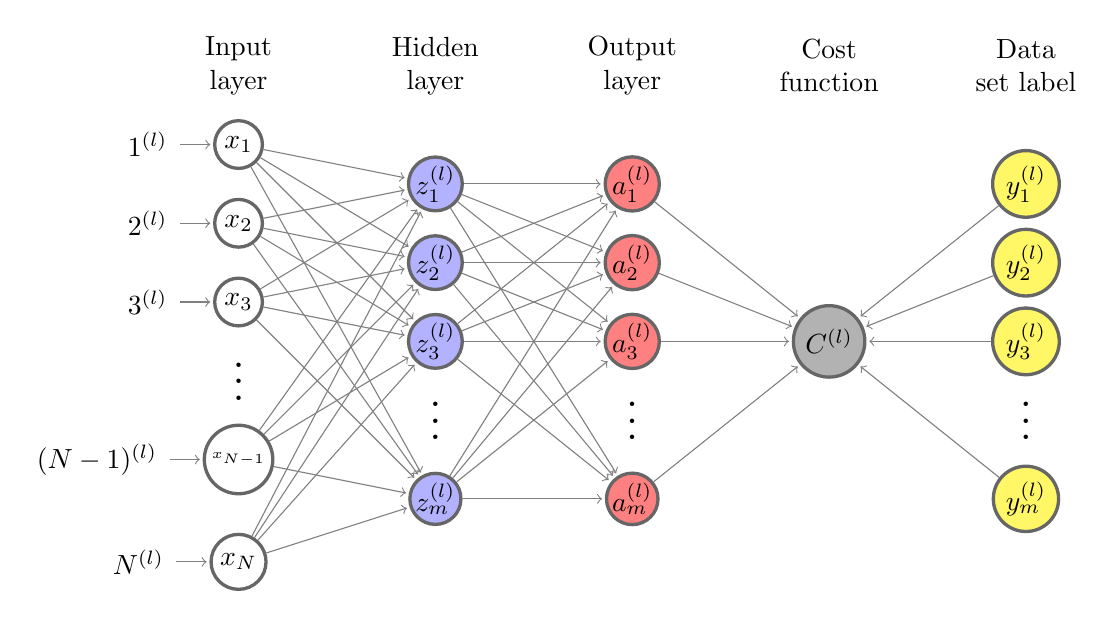
\begin{tikzpicture}[shorten >=1pt,->,draw=black!50, node distance=\layersep]
    \tikzstyle{every pin edge}=[<-,shorten <=1pt]
    \tikzstyle{neuron}=[circle,draw=black!60,fill=black!25,minimum size=17pt,inner sep=0pt, very thick]
    \tikzstyle{missing}=[draw=none, scale=1.5,text height=0.333cm,execute at begin node=\color{black}$\vdots$]
    \tikzstyle{input neuron}=[neuron, fill=white!50,inner sep=2pt];
    \tikzstyle{output neuron}=[neuron, fill=red!50];
    \tikzstyle{hidden neuron}=[neuron, fill=blue!30];
    \tikzstyle{cost neuron}=[neuron, fill=black!30,inner sep=2.4pt];
    \tikzstyle{label neuron}=[neuron, fill=yellow!60,inner sep=1.6pt];
    \tikzstyle{annot} = [text width=4em, text centered]

    % Draw the input layer nodes
    \foreach \name / \y in {1,2,3}
    	\path[yshift=0.5cm]
        	node[input neuron, pin=left:$\y^{(l)}$] (I-\name) at (0,-\y) {$x_\y$};
    \path[yshift=0.5cm]
    	node[missing] (I-4) at (0,-4) {};
    \path[yshift=0.5cm]
		node[input neuron, pin=left:$(N-1)^{(l)}$] (I-5) at (0,-5) {\tiny $x_{N-1}$};
	\path[yshift=0.2cm]
    	node[input neuron, pin=left:$N^{(l)}$] (I-6) at (0,-6) {$x_{N}$};
    
    % Draw the hidden layer nodes
    
    \foreach \name / \y in {1,2,3}
        \path[yshift=0.0cm]
            node[hidden neuron] (H-\name) at (\layersep,-\y cm) {$z_\y^{(l)}$};
    
    \path[yshift=0.0cm]
            node[missing] (H-4) at (\layersep,-4 cm) {};
    
    \path[yshift=0.0cm]
            node[hidden neuron] (H-5) at (\layersep,-5 cm) {$z_m^{(l)}$};

    % Draw the output layer
    
    \foreach \name / \y in {1,2,3}
        \path[yshift=0.0cm]
            node[output neuron] (O-\name) at (2*\layersep,-\y cm) {$a_\y^{(l)}$};
    
    \path[yshift=0.0cm]
            node[missing] (O-4) at (2*\layersep,-4 cm) {};
    
    \path[yshift=0.0cm]
            node[output neuron] (O-5) at (2*\layersep,-5 cm) {$a_m^{(l)}$};
            
     % Draw the Cost node
    
    \node[cost neuron, right of=O-3] (C) {$C^{(l)}$};
    
    % Draw the label layer
    
    \foreach \name / \y in {1,2,3}
        \path[yshift=0.0cm]
            node[label neuron] (Y-\name) at (4*\layersep,-\y cm) {$y_\y^{(l)}$};
    
    \path[yshift=0.0cm]
            node[missing] (Y-4) at (4*\layersep,-4 cm) {};
    
    \path[yshift=0.0cm]
            node[label neuron] (Y-5) at (4*\layersep,-5 cm) {$y_m^{(l)}$};


    % Connect every node in the input layer with every node in the
    % hidden layer.
    \foreach \source in {1,2,3,5,6}
        \foreach \dest in {1,2,3,5}
            \path (I-\source) edge (H-\dest);
	
    
    % Connect every node in the hidden layer with the output layer
    \foreach \source in {1,2,3,5}
        \foreach \dest in {1,2,3,5}
            \path (H-\source) edge (O-\dest);
	
	% Connect every node in the Output layer with the Cost node
    \foreach \source in {1,2,3,5}
        \path (O-\source) edge (C);	
	
	% Connect every node in the label layer with the Cost node
    \foreach \source in {1,2,3,5}
            \path (Y-\source) edge (C);	
	
    % Annotate the layers
    \node[annot,above of=I-1, node distance=1cm] (i1) {Input layer};
    \node[annot,right of=i1, node distance=\layersep] (hl) {Hidden layer};
    \node[annot,right of=hl, node distance=\layersep] (o1) {Output layer};
    \node[annot,right of=o1, node distance=\layersep] (c1) {Cost function};
    \node[annot,right of=c1, node distance=\layersep] (y1) {Data set label};
\end{tikzpicture}
\caption[Logistic regression diagram]{The single layer perceptron model of multinomial logistic regression.}
\label{LogisticRegressionDiagram}
\end{figure}
\subsubsection{Cost function}
In stochastic gradient descent, the cost function we will end up using in the below calculations are given by 
\begin{equation}
C = \sum\limits_{l=1}^{Batch\,size} C^{(l)}
\end{equation}
\subsubsection{Derivatives of the cost function}
We want to calculate the derivative of the new cost function with respect to the weights and biases. We will use these to calculate the step in the gradient descent:
$\textbf{W} = \textbf{W} -\eta \frac{d C}{d\textbf{W} }$ and $\textbf{b} = \textbf{b} -\eta \frac{d C}{d\textbf{b} }$. Using the chain rule, we can re-express this problem as
\begin{equation}\label{backprop1}
\frac{dC}{dw_{i,n}} = \sum_{j=1}^m \left (\frac{dC}{da_j} \right) \left (\frac{da_j}{dz_i} \right) \left(\frac{dz_i}{dw_{i,n}} \right )
\end{equation}
and
\begin{equation}\label{backprop2}
\frac{dC}{db_i} = \sum_{j=1}^m \left (\frac{dC}{da_j} \right) \left (\frac{da_j}{dz_i} \right) \left(\frac{dz_i}{db_i} \right )
\end{equation}
where $i \in [1,2,\cdots,m]$ and $n \in [1,2,\cdots,N]$. We can now proceed to solving each of these derivatives in turn:
\begin{equation}
\frac{dC^{(l)}}{da_j^{(l)}} = - \frac{y_j^{(l)}}{a_j^{(l)}},\,\,\, \frac{dz_i^{(l)}}{dw_{i,n}^{(l)}} =  x_n^{(l)},\,\,\, \frac{dz_i^{(l)}}{db_i^{(l)}} =  1.
\end{equation}
The derivative of the Softmax function $$\frac{da_j^{(l)}}{dz_i^{(l)}}$$ is $$a_j^{(l)}(\delta_{ji}-a^{(l)}_i)$$ but rather than this expression, we want to formulate the derivative as a $m \times m$ matrix:
\begin{equation}
\frac{d}{d \textbf{z}^{(l)}} \textbf{a}^{(l)} = (\textbf{a}^{(l)} \otimes \mathbf{1} )\circ (\mathbf{I} - \mathbf{1} \otimes \textbf{a}^{(l)}) = \textbf{M}
\end{equation}
where $\mathbf{1}$ is the $m \times 1$ one- vector, $ \mathbf{I} $ is the $m \times m$ unit matrix, $\otimes$ is the outer product and $\circ$ is the Hadamard product. The reason for this seemingly convoluted change in perspective, becomes apparent when we consider our equations \eqref{backprop1} and \eqref{backprop2}, which are now expressible (for a single datapoint) as
\begin{equation}\label{gradientW}
\frac{dC^{(l)}}{d\textbf{W}} =  \textbf{M}\cdot(- \textbf{y}^{(l)}\oslash \textbf{a}^{(l)}) \textbf{x}^{(l)}
\end{equation}
and
\begin{equation}\label{gradientb}
\frac{dC^{(l)}}{d\textbf{b}} =  \textbf{M}\cdot(- \textbf{y}^{(l)}\oslash \textbf{a}^{(l)}) 
\end{equation}
where $\oslash$ is the Hadamard division. With the gradients in hand, we can now optimize the weights and biases through gradient descent.

\subsubsection{Algorithm}
The algorithm for Logistic regression goes as follows. We make an initial guess for the weights and biases. Using these and a data point we calculate the activation function. This is then used, together with the same data point in calculating the gradient of the cost function, which is used to calculate the new, optimized parameters $\textbf{W}$ and $\textbf{b}$.
\begin{figure}[H]
\begin{center}
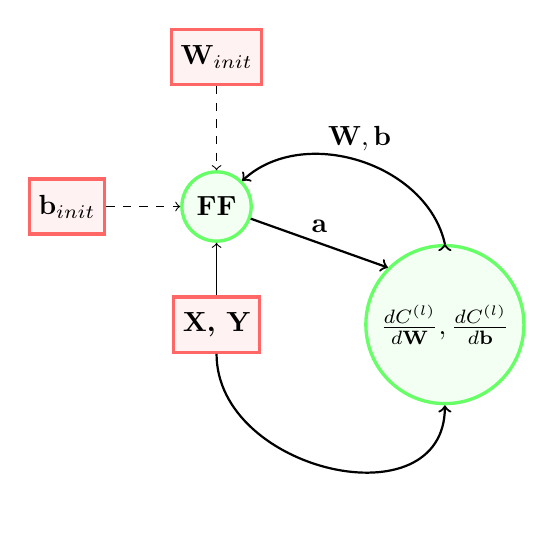
\begin{tikzpicture}[
roundnode/.style={circle, draw=green!60, fill=green!5, very thick, minimum size=7mm},
squarednode/.style={rectangle, draw=red!60, fill=red!5, very thick, minimum size=7mm},]
%Nodes
\node[squarednode]      (Winit)                              {$\textbf{W}_{init}$};
\node[roundnode, yshift = -0.9cm]      (FF)  [below of = Winit]{$\textbf{FF}$};
\node[squarednode, xshift = -0.9cm]      (binit)  [left of = FF]{$\textbf{b}_{init}$};
\node[squarednode, yshift = -0.5cm]      (XY)  [below of = FF]{$\textbf{X, Y}$};
\node[roundnode, xshift = 1.9cm]      (grad)  [right of = XY]{$\frac{dC^{(l)}}{d\textbf{W}},\frac{dC^{(l)}}{d\textbf{b}}$};

%Lines
\draw[->,dashed] (Winit.south) -- (FF.north);
\draw[->,dashed] (binit.east) -- (FF.west);
\draw[->] (XY.north) -- (FF.south);

\path[->,draw,thick] (FF) edge node[above] {$\textbf{a}$} (grad.north west);

\draw[->,thick] (XY.south) .. controls +(down:15mm) and +(down:15mm) .. (grad.south);

\path[->,draw,thick] (grad.north) edge [bend right=60] node[above] {$\textbf{W},\textbf{b}$} (FF.north east);
\end{tikzpicture}
\end{center}
\caption[Logistic regression algorithm]{The algorithmic structure of logistic regression. Red squares represent variables that enter the algorithm. Green circles represent computations and dashed arrows means the output is used once.}
\label{LogisticRegressionFlowchart}
\end{figure}
This process continues until either a given number of iterations have taken place, or the Softmax function produces an output error within a given tolerance. 
\subsection{Gradient Descent Methods}
One way to find the minima, both local and global, of a (multivariable) function, one can use the method of gradient descent. Simply speaking, this is done by iteratively changing the parameters in order to minimize a cost function \citep{handsOnMachineLearning}. As the gradient of a function always shows towards the point of steepest descent, following the gradient in the opposite direction will lead to a minimum. In both regression and classification problems, the function to be minimized is the cost function. In terms of linear regression, the cost function is the MSE function (possibly with additional regularization). The gradient is simply a vector containing the partial derivatives with respect to each coefficient $\beta_i$.\\
For OLS and Ridge regression, we have that 
\begin{equation}
     \nabla_\beta C(\beta)=\frac{2}{m} \left[X^T \left(X\beta-y\right)\textcolor{red}{+\lambda\beta} \right]
\end{equation}
where C is the cost function, X is the design matrix and m is the number of inputs. The \textcolor{red}{red} part is only added for Ridge Regression. \\
After having an initial guess for the values $\beta^0$, The values $\beta$ are then be updated iteratively by following the gradient in the opposite direction:
\begin{equation}\label{Updatescheme}
\beta^{i+1}=\beta^{i}- \gamma \nabla_\beta C(\beta^{i})
\end{equation}
where we introduced the learning rate $\gamma$. The learning rate $\gamma$ needs to be chosen in such a way that it is not too large (which can lead to divergent behaviour), but not too small either (which can lead to an extremely slow convergence). This is done either until convergence is reached, or for a given number of iterations, called \textit{epochs}.
\subsubsection{Stochastic Gradient Descent Methods}
Because calculating the gradient of every parameter $\beta$ can be rather costly for large data sets, the gradient can be approximated by the gradient at only one input variable which is chosen randomly. This introduces randomness and erratic behaviour to the way the minimum is found. It is hence likely that the minimum is well approximated, but not exact \citep{handsOnMachineLearning}. However, the advantage is that the stochastic method can "jump out of" local minima and find the global minimum. One closely related method is Mini-batch gradient descent, where the gradient is approximated by the gradient at several, but not all, randomly chosen input variables. This leads to a less erratic behaviour, but is still computationally cheaper than Gradient Descent.
There are several ways to implement the actual gradient descent. It is useful to adapt the learning rate $\gamma$ as the program proceeds - starting with a comparatively large learning rate, the algorithm can  leave local minima and proceed to the global minimum, while the learning rate is gradually reduced to get better convergence. In the following, three methods of varying complexity will be introduced.
\paragraph*{"Naive" Stochastic Gradient Descent} has a constant learning rate $\gamma$, and the parameters $\beta$ are just updated by \eqref{Updatescheme} where the gradient is approximated. While this is easy to implement, has only one parameter ($\gamma$) to be fine tuned, and is cheap to calculate, the non-adaptive learning rate $\gamma$ can lead to sub-optimal convergence.
\paragraph*{Decaying $\gamma$}
- A simple way to make $\gamma$ get smaller gradually is to implement a gradual decay. Defining
\begin{equation}
\gamma_t=\frac{t_0}{t_1+t}
\end{equation}
where $t_0$ and $t_1$ are initialization parameters and t is updated as $t=e\cdot m+i$ where $e$ is the actual epoch, $i$ is the actual mini batch and $m$ is the number of mini batches. The update scheme remains the same \eqref{Updatescheme}, just that $\gamma_t$ is used instead of a fixed $\gamma$. While this method has the advantage that $\gamma_t$ gradually gets reduced, eventually $\gamma$ gets so small that the steplength gets so small that no convergence is reached.
\paragraph*{RMSProp} describes a method where the learning rate is reduced gradually by accumulating the gradients from previous iterations, however, unlike the previous method, the impact of previous iterations decays exponentially. The update scheme is described as 
\begin{equation}
\begin{split}
    &\bm{s}^{i+1}=\alpha \bm{s}^{i}+(1-\alpha) \nabla_\beta C(\bm{\beta^{i}})* \nabla_\beta C(\bm{\beta^{i}}) \\
   &\bm{\beta}^{i+1}=\bm{\beta}^{i}-\gamma C(\bm{\beta^{i}}) / \sqrt{\bm{s}^{i+1}+e}
\end{split}
\end{equation}
where * and / refer to element-wise multiplication and division, respectively. In this article, we chose the default value $\alpha=0.9$, while $e=10^{-8}$ simply has the purpose of avoiding zero division.
\paragraph*{ADAM} is a method related to RMSProp, and is a shortcut for \textit{adaptive momentum estimation}. It combines features of RMSProp and a method called Momentum optimization (see for example \citep{MortenLectureNotes}) - it keeps track of the average of past gradients, but also the average of past gradients squared, and both are to decay exponentially. The update scheme is described as 
\begin{equation}
\begin{split}
    & \bm{m}^{i+1}=[\alpha_1\bm{m}+(1-\alpha_1) \nabla_\beta C(\bm{\beta^{i}})](1-\alpha_1^T)^{-1}\\
    &\bm{s}^{i+1}=\alpha_2 \bm{s}^{i}+(1-\alpha_2) \nabla_\beta C(\bm{\beta^{i}})* \nabla_\beta C(\bm{\beta^{i}})(1-\alpha_2^T)^{-1} \\
   &\bm{\beta}^{i+1}=\bm{\beta}^{i}-\gamma\bm{m}^{i+1} / \sqrt{\bm{s}^{i+1}+e}
\end{split}
\end{equation}
where * and /  again refer to element-wise multiplication and division, respectively; and T stands for the number of iterations (starting at 1). In this article, we chose the default values $\alpha_1=0.9$ and $\alpha_2=0.99$, while $e=10^{-8}$ simply has the purpose of avoiding zero division.
\subsection{Neural networks}
A Feed Forward Neural Network consists first of an input layer with neurons corresponding to each predictor in a data set. Then one or more hidden layers with neurons with weighted connections between every neuron in the two adjacent layers. Every neuron in the hidden layers are equipped with a bias, determining in a sense the activation threshold for that neuron. Additionally the weighted and biased sum of each neuron (with respect to the previous layer) is passed through an activation function. Finally, the activations reach the last hidden layer which is connected to the output layer, consisting of however many neurons needed to occupy the range of outputs we consider. 
\subsubsection{Back propagation}
A neural network is parametrized by a set of Weight's and biases. When the cost function is being optimized, the weights and biases belonging to every neuron in the network have to be updated. The cost function only "sees" the activation from the output layer of the network. We therefore need to determine how the cost function changes with respect to the weights in all the hidden layers. Fortunately, we can accomplish this through the chain rule.\\\\ We have for the output layer of the network that through the chain rule we can write
\begin{equation}\label{BreakerOfChains}
\frac{\partial C}{\partial \textbf{W}^{(L)}} = \frac{\partial \textbf{z}^{(L)}}{\partial \textbf{W}^{(L)}}\frac{\partial \textbf{a}^{(L)}}{\partial \textbf{z}^{(L)}}\circ \frac{\partial C}{\partial \textbf{a}^{(L)}}
\end{equation}

It's quick to check that $\frac{\partial \textbf{z}^{(L)}}{\partial \textbf{W}^{(L)}} = \textbf{a}^{(L-1)}$. The remaining derivatives in the expression depend on the choice of activation function and cost function but are generally easy to calculate. We can also introduce the new variable $\delta^{(L)} = \frac{\partial \textbf{a}^{(L)}}{\partial \textbf{z}^{(L)}}\circ
\frac{\partial C}{\partial \textbf{a}^{(L)}}$. Equation \eqref{BreakerOfChains} becomes 
\begin{equation}
\frac{\partial C}{\partial \textbf{W}^{(L)}} = \textbf{a}^{(L-1)}\delta^{(L)}.
\end{equation}
This is all well and good, but it doesn't tell us how we ought to change the weights in all the preceding layers. We'll introduce another expression, returning partially to equation \eqref{BreakerOfChains}, we see that can also, simply treat $\delta^{(l)} = \frac{\partial C}{\partial \textbf{z}^{(l)}}$ rather than the Hadamard product. We'll use the chain rule again, but now to see how the cost function changes with respect to the succeeding layer:
\begin{equation}
\delta^{(l)} =\sum_k \frac{\partial C}{\partial z_k^{(l+1)}}\frac{\partial z_k^{(l+1)}}{\partial \textbf{z}^{(l)}}
\end{equation}
This gives an equation that can be iterated all the way from the last to the first hidden layer, and we can use it to update the weights and biases (the bias follows similarly). 
\subsubsection{Feed Forward}
After every new weight and bias in the network has been calculated, it's simply a matter of calculating the activations belonging to each layer from the first to the last layer in the network (since the activation of one layer depends on the activations in the preceding layer). After this process the network has a slightly altered cost function to optimize and the process repeats. 
\subsubsection{Activation functions}
As described in the previous to subsections, the activation function is one of the core elements in Neural Networks. In this project, we implemented the following four activation functions for activation between the input layer and the first hidden layer as well as between all hidden layers. 
\paragraph*{sigmoid function} - The sigmoid function, defined as $\sigma(x)=\frac{e^x}{e^x-1}$, outputs function values between 0 and 1 for all inputs. 
\paragraph*{tanh} - The tanh function, which can be expressed in terms of the sigmoid function $tanh(x)=2\sigma(2x)-1$, can take functions between -1 and 1. Unlike the sigmoid function, it maps negative inputs to negative function values, while 0 is mapped to 0.
\paragraph*{ReLU} -The ReLU function (\textit{Rectified Linear Unit}) is defined as $ReLU(x)=x^+$ (x if x is positive, zero otherwise). Unlike the tanh function and the sigmoid function, it does not suffer from vanishing gradients when the input values are large. It has been shown \citep{surpremeRELU} that rectifiers can give better results in Machine learning, especially depper networks, than the sigmoidal functions.
\paragraph*{LeakyReLU} - The LeakyReLU function is defined as $LeakyReLU(x)=max(x,\alpha x)$ where $\alpha=0.01$ (though other values are possible, too). Positive values are hence mapped to themselves, whereas negative input values are mapped to $\alpha x$. Unlike the ReLU function, it has nonzero output for negative input values too, and the gradient vanishes nowhere, improving the problem of "dying" neurons.\\\\
For the output, we used no activation function (Regression) or the Softmax activation function (Classification). 
\paragraph*{Softmax function} - The Softmax function defined in equation \eqref{softmax} is a generalization of the Logistic function (sigmoid), and is used to classify more than two categories.
\subsection{Data sets}
\subsubsection{Regression: Terrain Data}
For the regression analysis, we used the same data as in \citep{Project1} - a black-and white image with resolution $3601 \times 3601$ pixel which represents an area in the Taebaek Mountains in South Korea with a total surface area of $3601 \times 3601km^2$ , hence each square kilometer is represented as one pixel, where colour intensity represents the height (black equals height at sea level).
\subsubsection{Classification: MNIST data set}
For classification, we use the MNIST data set, a data set consisting of 70.000 handwritten digits between 0 and 9, represented as a picture with resolution $28\times28$ pixel \citep{lecun2010mnist}. In this article however we used Scikit Learn's variant of the MNIST data set, which consists of 1797 elements with resolution $8\times8$ pixel. 
\section{Computational implementation}

\subsection{Multinomial logistic regression}
We have chosen classification of handwritten digits in an $8\times 8$ grid of pixels, as the classification problem. To implement this, the $(8\times 8)\times L$ pixel data is flattened into a $(L \times 64)$ matrix with $L$ being the number of datapoints. The image labels, originally a $(L \times 1)$ array of digits $0$ through $9$, is converted into a One- hot matrix representation of shape $(L \times 10)$. The computational implementation of Softmax regression follows from the illustrations in figures \ref{LogisticRegressionDiagram} and \ref{LogisticRegressionFlowchart}. 

\subsubsection{Numerically stable variants}
The Softmax function defined in \eqref{softmax}, is inherently prone to overflow. We can resolve this by making a small change:
\begin{equation}
a_i= \frac{e^{z_i}}{\sum_{j=1}^{m} e^{z_j}} \cdot \frac{e^{-c}}{e^{-c}} = \frac{e^{z_i-c}}{\sum_{j=1}^{m} e^{z_j-c}}
\end{equation}
where we choose $c = \max \{ z_i : i \in [1,2,\cdots ,m]\} $. In this way we ensure that the function does not overflow, as the exponent is always smaller than zero. Only a unique set of circumstances could cause this expression to be numerically unstable, for example if the sum in the denominator is ever zero.\\Additionally, the Hadamard division used to calculate the gradients in equations \eqref{gradientW} and \eqref{gradientb} receives a tiny addition of $10^{-15}$ in the denominator to avoid division by zero.

\subsection{Neural network}
\subsubsection{Numerically stable variants}
We used the same Softmax function as for multinomial logistic regression. For the sigmoid function, we used Scipy's \citep{SciPy} expit function.
\subsubsection{Setting up weights and biases for the neural network}
As there is no clear rule how to set up weights and biases, other than that they should be initialized with a non-zero value, we first tried to set up the weights with a mean zero normal distribution with a small standard deviation $\sigma\approx0.01$. However, we found that this yielded undesirable results, which made that especially ReLU and LeakyReLU gave unpredictable behaviour where the activation function gave very high numbers, eventually leading to numerical instability and overflow. Hence, we decided to follow the approach described in \cite{DelvingDeep}, where the weights are initialized randomly, following a mean zero normal distribution with standard deviation $\sigma=\sqrt{2/n\_inputs}$ where n\_inputs here refers to the batch size. The biases were simply initialized with a small nonzero number - $0.001$.
\subsubsection{Functionality of the Neural Network}
We designed a flexible Neural Network that works with any amount of hidden layers and any amount of neurons per hidden layer. It works with both classification and regression, using the softmax function as activation function for the output layer for classification, and simply the linear function $f(x)=x$ for the regression case. 
\subsubsection{Adapting the Neural Network for Classification}
Very little is needed to apply the neural network in classification problems. The dataset needs to be flattened (For this type of neural network, other types may exploit patterns that are destroyed in this process) such that each datapoint can enter the network as a vector. The labels should be converted (if not already) to the corresponding One- Hot representation.\\Beyond this, the output layer of the network needs to be equipped with either the Sigmoid- or Softmax activation function. There is always the choice of cost function which, invariably for our purposes should be the Cross- Entropy cost function.
\section{Results}
\subsection{Comparison of SGD methods for OLS}
Figure \ref{fig:DifferentSGD} shows, for a given OLS problem, the test MSE as a function of the learning rate $\eta$ for a fixed number of epochs \& a fixed batch size; the test MSE as a function of the number of epochs for a fixed learning rate \& a fixed batch size; and the test MSE as a function of batch size for a fixed number of epochs and a fixed learning rate. 

\begin{figure}[H]
\centering
\includegraphics[width=0.95\textwidth]{OLS_error_SGD_idealLearningRate.pdf}
\caption[Test MSE Different SGD methods for OLS]{The simple SGD method (titled SGD), RMSProp, ADAM and decaying $\eta$ as functions of the learning rate $\eta$ (top left), the number $t_1$ (top right), the number of epochs (down left), and different batch sizes (down right). The number of data points is $N=2000$, the polynomial degree used is $deg=10$. For the top two plots, a batch size of 16 and and epoch of 1000 were chosen. The lower to plots use the ideal parameters $\eta$ and $t_1$ which were chosen based on the ideal values from first two plots. No bootstrapping or cross-validation was performed.}\label{fig:DifferentSGD}
\end{figure}
As one can see, the number of epochs and the learning rate make a huge difference when it comes to approximating the analytical solution. For the decay-SGD and the simple SGD (titled SGD), the curves are truncated because too big or too small values lead to NaN-values. This shows that the ideal learning rate is dangerously close to a too high learning rate, leading to completely wrong numbers or even NaN-values. Similar observations can be done for both ADAM and RMSProp, but the change is not as drastic for these methods.\\ 
As expected, the number of epochs lead to increased error reduction for all methods. However, even though the number of epochs grows exponentially, the error reduction slows down and even ceases. This is hence a computationally expensive way of reducing the extra error. As the learning rate was chosen to be ideal for 1000 epochs, we also see that, at least with ADAM, the error actually increases - this might be due to over-fitting, or leaving the reached minimum.\\
The number of batches does not seem to have a large impact on the quality of the fit for  ADAM, but we observe that the simple SGD method and RMSProp work best with small batch sizes. This might be because these methods work best when making many "small hops" instead of several larger hops.\\
One can see that the choice of method has a large impact on how fast the error is reduced. RMSProp and ADAM seem to be slightly superior to the simple SGD in terms of convergence to the true MSE, however their biggest advantage is that they are more stable and have "broader" ideal learning rates. This is not surprising as these methods were developed for this purpose. ADAM seems to be better at dealing with higher epochs than RMSProp though. The decay-fit method, while giving results as good as RMSProp and ADAM for ideal parameters, is too unstable to be used in practice - small fluctuations in the parameters lead to completely wrong values. It is also harder to tweak several parameters. 
Figure \ref{fig:DifferentSGD_fixedEta} contains the same plots as figure \ref{fig:DifferentSGD}, however, the learning rates $\eta$ were chosen so that they didn't exceed a value of 0.1. This is more difficult to do for the decay method, which we left unchanged. One can see that this leads to a slightly different behaviour. The convergence is, not surprisingly, slower, but the methods behave slightly less erratic. That way, the error keeps reducing as the number of epochs increases, but it takes more epochs to get it to the same level as before. Also, the error now increases for larger batch sizes for all methods, including ADAM. In this implementation, a larger batch size has no computational advantages, however, for the Neural Network later, larger batch sizes give increased run time. 
\begin{figure}[H]
\centering
\includegraphics[width=0.95\textwidth]{OLS_error_SGD_fixedLearningRate.pdf}
\caption[Test MSE Different SGD methods for OLS (fixed $\eta$)]{The simple SGD method (titled SGD), RMSProp, ADAM and decaying $\eta$ as functions of the learning rate $\eta$ (top left), the number $t_1$ (top right), the number of epochs (down left), and different batch sizes (down right). The number of data points is $N=2000$, the polynomial degree used is $deg=10$. For the top two plots, a batch size of 16 and and epoch of 1000 were chosen. The lower to plots use the ideal parameters $\eta$ and $t_1$ which were chosen based on the first two plots, however, $\eta$ was chosen so that $\eta \leq 0.1$ as larger numbers lead to instability later on. No bootstrapping or cross-validation was performed.}\label{fig:DifferentSGD_fixedEta}
\end{figure}
\subsubsection{Comparison of SGD methods for Ridge regression}
We repeated the same analysis as above with Ridge regression, only varying the learning rate and the regularisation parameter, keeping the batchsize fixed (16), as well as the number of epochs (1000). We chose a high polynomial degree where OLS is inferior to Ridge regression. The results can be seen in figure \ref{fig:DifferentSGDRIDE} in the appendix. The difference between the methods is baffling. We see that simple SGD gives NaN-values for too high learning rates, as before. RMSProp and ADAM, too, give worse results as the learning rate increases, but to a much lesser degree than simple SGD. As we did not perform Cross Validation, these numbers are only qualitatively correct, but we see that all methods, given the ideal parameters are chosen, can get very close to the analytical result. ADAM performs best and manages to come close to the analytical solution, however, both RMSProp and the simple SGD method get quite close, too. We see that regularization gives improved values for Stochastic Gradient Descent methods, to, as very small regularization parameters $\lambda$ yield worse test errors than the optimal parameters. We see however that the error is always larger than the ideal test error, implying that Stochastic Gradient Descent methods can get quite close, but not exactly equal to the ideal analytical parameters, at least not with the chosen parameters. 
\subsection{FFNN for Regression}
We used randomly selected points from the terrain data \citep{Project1} to create a fit using both OLS and Ridge Regression, as well as the Neural Network.
\subsubsection{Comparing the FFNN to Scikit-learn}
We tested the quality of our Neural Network with N=2000 randomly selected data points and a polynomial degree of 10. We chose 200 as batch size and 1000 epochs. We used one hidden layer with 100 neurons. The sigmoid function was used as activation function for the hidden layer, and simple gradient descent was used. Figure \ref{fig:ScikitLearn_1} plots the test and train error as function of the regularization parameter $\lambda$ and the error learning rate $\eta$. Using OLS, we found 28272 for the test MSE and 24758 for the train MSE, for comparison. We also compared this to Scikit-learn 's MLPRegressor function \citep{scikit-learn}, which are included in figure \ref{fig:ScikitLearn_1}.
\begin{figure}[H]
\centering
\includegraphics[width=1.05\textwidth]{scikit_own_1b1_logisticsgd200010.pdf}
\caption[Scikit-learn  and own FFNN with 1 layer]{Train and test MSE \underline{divided by 1000} as function of the learning rate $\eta$ and the regularization parameter $\lambda$ for our own Neural Network and Scikit-learn 's MLPRegressor function. We used 2000 data points (randomly selected), a polynomial degree of 10, a batch size of 200, 1000 epochs, one hidden layer with 100 neurons, simple SGD as gradient descent method and the sigmoid function as activation function between the layers. Values exceeding 100,000 are excluded from the plot. We used 5-fold Cross Validation to estimate the errors.} \label{fig:ScikitLearn_1}
\end{figure}
First of all, we see that both Scikit-learn and our own Neural Network outperform OLS (and Ridge regression, which gives identical values here). Values like that were not possible to obtain only using Linear Regression for that amount of data points \citep{Project1}, indicating that Neural Networks can give superior results to Linear Regression methods. This comes however at the cost of not obtaining a nice function expression (it is up to the reader to decide if a multivariate polynomial of degree 10 is a nice function expression - but the number of parameters is bearable) with a meaning behind it. \\
We see that our algorithm gave superior values to Scikit-learn. This is supposedly due to a different implementation of the SGD-algorithm, as is clear as the ideal parameters for the learning rate differ by one magnitude. Finally, we see that choosing wrong parameters ends up giving completely horrendous results, meaning that tweaking both the regularization parameter and the learning rate is necessary.
\subsubsection{Impact of number of hidden layers}
Exactly the same analysis as before (compare figure \ref{fig:ScikitLearn_1}) was done, this time using two hidden layers with 100 neurons each. The results can be seen in figure \ref{fig:ScikitLearn_2}.
\begin{figure}[H]
\centering
\includegraphics[width=1.05\textwidth]{scikit_own_2b1_logisticsgd200010.pdf}
\caption[Scikit-learn  and own FFNN with 2 layers]{Train and test MSE \underline{divided by 1000} as function of the learning rate $\eta$ and the regularization parameter $\lambda$ for our own Neural Network and Scikit-learn 's MLPRegressor function. We used 2000 data points (randomly selected), a polynomial degree of 10, a batch size of 200, 1000 epochs, two hidden layers with 100 neurons each, simple SGD as gradient descent method and the sigmoid function as activation function between the layers. Values exceeding 100,000 are excluded from the plot. We used 5-fold Cross Validation to estimate the errors.} \label{fig:ScikitLearn_2}
\end{figure}
We see that adding the second layer gives even better results than just using one hidden layer. This indicates that using more layers can further reduce the error. Again, our Neural Network outperforms Scikit learn, but the difference is smaller than with just one single layer.\\We also run the same analysis with a polynomial degree of 20. The results can be seen in figure \ref{fig:ScikitLearn_3} in the appendix. Here, OLS fails due to a too high variance. Ridge regression can be used though and gave a test error of 24312, while our own Neural Network with 2 layers gave a test error of 20251 (which is slightly worse than the error produced by Scikit Learn, which is 20043. The test error for the neural network has hence increased - we suppose that the increased amount of parameters leads to a slower convergence rate, it might be possible that increasing the number of iterations might lead to better parameters. 
\subsubsection{Comparison between ADAM, RMSProp \& simple SGD}
Figure \ref{fig:ADAMvsRMSProp} contains the train and the test MSE using ADAM \& RMSProp as stochastic gradient descent methods using our own FFNN. The parameters are identical to the ones in figure \ref{fig:ScikitLearn_2}, that is, two hidden layers with 100 neurons each. 
\begin{figure}[H]
\centering
\includegraphics[width=1.05\textwidth]{ADAM_RMSProp_2b1_logisticRMSProp200010.pdf}
\caption[ADAM \& RMSProp with 2 layers]{Train and test MSE \underline{divided by 1000} as function of the learning rate $\eta$ and the regularization parameter $\lambda$ for our own Neural Network using ADAM and RMSProp. We used 2000 data points (randomly selected), a polynomial degree of 10, a batch size of 200, 1000 epochs, two hidden layers with 100 neurons each and the sigmoid function as activation function between the layers. Values exceeding 100,000 are excluded from the plot. We used 5-fold Cross Validation to estimate the errors.} \label{fig:ADAMvsRMSProp}
\end{figure}
We see that the methods are generally similar and give similar test and train errors for similar parameters. However, ADAM copes better with too high learning rates and the results at high learning rates, albeit much worse than with good parameters, do not explode. ADAM also surpasses simple SGD in the sense that the lowest obtained test MSE is slightly lower, while RMSProp is on pair. 
\subsubsection{Impact of activation function}
As ADAM has given the best test results, we used ADAM as stochastic gradient method and compared the impact of the four different activation functions ReLU, tanh, sigmoid \& LeakyReLU. This can be seen in figure \ref{fig:ADAMdifferentActivationFunctions}.
\begin{figure}[H]
\centering
\includegraphics[width=1.05\textwidth]{Four_activations2ADAM200010.pdf}
\caption[Different activation functions]{Test MSE \underline{divided by 1000} as function of the learning rate $\eta$ and the regularization parameter $\lambda$ for our own Neural Network using ADAM. We used 2000 data points (randomly selected), a polynomial degree of 10, a batch size of 200, 1000 epochs, two hidden layers with 100 neurons each and the activation function stated in the title between the layers. Values exceeding 100,000 are excluded from the plot. We used 5-fold Cross Validation to estimate the errors.} \label{fig:ADAMdifferentActivationFunctions}
\end{figure}
As we see, the tanh function gave by far the best results with a test MSE below $18,000$, followed by the sigmoid function. This does not show that the tanh function is the best activation function, but that the tanh function in this case, with the given amount of layers and chosen parameters as well as the number of epochs, performs best. It is interesting to see that both the ReLU and the LeakyReLU activaton functions seem to be more "forgiving" to different learning rates and regularization parameters, as a larger part of the 2D table appears blue, indicating small values, than with the tanh function \& the sigmoid function.\\

For comparison, we run a small test with 4 hidden layers of sizes (100,100,50,50) (in that order, where the output layer is to the right), but only 100 epochs due to the high time usage. The result can be found in figure \ref{fig:4layers} in the appendix where the test error is portrayed for all 4 methods. From this graph, we see that ReLU \& LeakyReLU perform much better for this deeper neural network. Not only is the smallest test error lower, the methods are much more stable too, in the sense that the both ReLU and LeakyReLU give good results for much more values of the learning rate and the regularization parameter, whereas tanh and especially the sigmoid function are very narrow. Figure \ref{fig:2layers} in the appendix is also run with only 100 epochs, but has only 2 hidden layers. Here, the sigmoid function and the tanh function are superior, however the test error achieved with both the LeakyReLU and ReLU and 4 layers is lower than the test error from the tanh function and two layers (and all sigmoid function values except for one), indicating that the ReLU/LeakyReLU can indeed give better results.


\subsection{FFNN for Digit Classification}
\subsubsection{Comparing the FFNN to Scikit- learn}
For comparison, we chose the Scikit Learn MLPClassifier. Parametrized with the ADAM solver using $\beta_1 = 0.9$ and $\beta_2 = 0.99$, an architecture of [100, 100, 50, 50], 100 epochs, a batch size of 100, learning rate of 0.001 and L2 regularization parameter of 0.0001. This is as close as possible to our own implementation using the RELU solver. Both results we found using 4-fold cross validation. The results of our implementation can be found in figure \ref{NN_activation}. Using the parameters above, this model accomplishes a testing accuracy of 97\%. The equivalent MLPClassifier function accomplishes a testing accuracy of 96\%. Within the scope of random deviation, these results are essentially the same. This is a good indication that we have correctly implemented the Neural network and applied it to classification.



\subsubsection{Impact of Network Architecture}
To examine the impact that the choice of network architecture makes, we decided on four archetypes. Two variations on the single layer perceptron model, to see the impact of increasing the number of neurons. Additionally, a more square architecture and what I'll decide to call a thin and deep architecture. All of which are shown in figure \ref{NNarchitectures} below.

\begin{figure}[H]


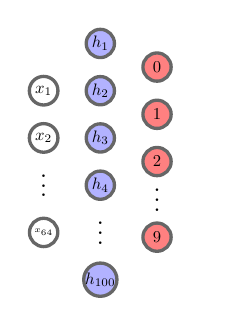
\begin{tikzpicture}[thick,scale=0.6, every node/.style={scale=0.6}][shorten >=1pt,->,draw=black!50, node distance=\layersep]
    \tikzstyle{every pin edge}=[<-,shorten <=1pt]
    \tikzstyle{neuron}=[circle,draw=black!60,fill=black!25,minimum size=17pt,inner sep=0pt, very thick]
    \tikzstyle{missing}=[draw=none, scale=1.5,text height=0.333cm,execute at begin node=\color{black}$\vdots$]
    \tikzstyle{dead}=[draw=none, scale=1.5,text height=0.333cm]
    \tikzstyle{input neuron}=[neuron, fill=white!50,inner sep=2pt];
    \tikzstyle{output neuron}=[neuron, fill=red!50];
    \tikzstyle{hidden neuron}=[neuron, fill=blue!30];
    \tikzstyle{cost neuron}=[neuron, fill=black!30,inner sep=2.4pt];
    \tikzstyle{label neuron}=[neuron, fill=yellow!60,inner sep=1.6pt];
    \tikzstyle{annot} = [text width=4em, text centered]

    % Draw the input layer nodes
    \foreach \name / \y in {1,2}
    	\path[yshift=-1.0cm]
        	node[input neuron] (I-\name) at (0,-\y) {$x_\y$};
    \path[yshift=-1.0cm]
    	node[missing] (I-3) at (0,-3) {};
    \path[yshift=-1.0cm]
		node[input neuron] (I-4) at (0,-4) {\tiny $x_{64}$};
    
    % Draw the hidden layer nodes
    
    \foreach \name / \y in {1,2,3,4}
        \path[yshift=0.0cm]
            node[hidden neuron] (H-\name) at (\layersepSmall,-\y cm) {$h_\y$};
    
    \path[yshift=0.0cm]
            node[missing] (H-5) at (\layersepSmall,-5 cm) {};
    
    \path[yshift=0.0cm]
            node[hidden neuron] (H-6) at (\layersepSmall,-6 cm) {$h_{100}$};

    % Draw the output layer
    
    \foreach \name / \y in {0,1,2}
        \path[yshift=-1.5cm]
            node[output neuron] (O-\name) at (2*\layersepSmall,-\y cm) {$\y$};
    
    \path[yshift=-0.3cm]
            node[missing] (O-4) at (2*\layersepSmall,-4 cm) {};
    
    \path[yshift=-0.1cm]
            node[output neuron] (O-5) at (2*\layersepSmall,-5 cm) {$9$};
         
    %Draw empty neuron for x- seperation   
    \path[yshift=-0.1cm]
            node[dead] (D-5) at (3*\layersepSmall,-5 cm) {};
            
\end{tikzpicture}
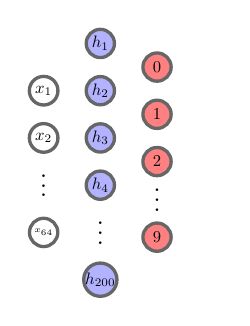
\begin{tikzpicture}[thick,scale=0.6, every node/.style={scale=0.6}][shorten >=1pt,->,draw=black!50, node distance=\layersep]
    \tikzstyle{every pin edge}=[<-,shorten <=1pt]
    \tikzstyle{neuron}=[circle,draw=black!60,fill=black!25,minimum size=17pt,inner sep=0pt, very thick]
    \tikzstyle{missing}=[draw=none, scale=1.5,text height=0.333cm,execute at begin node=\color{black}$\vdots$]
    \tikzstyle{input neuron}=[neuron, fill=white!50,inner sep=2pt];
    \tikzstyle{output neuron}=[neuron, fill=red!50];
    \tikzstyle{hidden neuron}=[neuron, fill=blue!30];
    \tikzstyle{dead}=[draw=none, scale=1.5,text height=0.333cm]
    \tikzstyle{cost neuron}=[neuron, fill=black!30,inner sep=2.4pt];
    \tikzstyle{label neuron}=[neuron, fill=yellow!60,inner sep=1.6pt];
    \tikzstyle{annot} = [text width=4em, text centered]

    % Draw the input layer nodes
    \foreach \name / \y in {1,2}
    	\path[yshift=-1.0cm]
        	node[input neuron] (I-\name) at (0,-\y) {$x_\y$};
    \path[yshift=-1.0cm]
    	node[missing] (I-3) at (0,-3) {};
    \path[yshift=-1.0cm]
		node[input neuron] (I-4) at (0,-4) {\tiny $x_{64}$};
    
    % Draw the hidden layer nodes
    
    \foreach \name / \y in {1,2,3,4}
        \path[yshift=0.0cm]
            node[hidden neuron] (H-\name) at (\layersepSmall,-\y cm) {$h_\y$};
    
    \path[yshift=0.0cm]
            node[missing] (H-5) at (\layersepSmall,-5 cm) {};

    \path[yshift=0.0cm]
            node[hidden neuron] (H-6) at (\layersepSmall,-6 cm) {$h_{200}$};

    % Draw the output layer
    
    \foreach \name / \y in {0,1,2}
        \path[yshift=-1.5cm]
            node[output neuron] (O-\name) at (2*\layersepSmall,-\y cm) {$\y$};
    
    \path[yshift=-0.3cm]
            node[missing] (O-4) at (2*\layersepSmall,-4 cm) {};
    
    \path[yshift=-0.1cm]
            node[output neuron] (O-5) at (2*\layersepSmall,-5 cm) {$9$};
    
    %Draw empty neuron for x- seperation   
    \path[yshift=-0.1cm]
            node[dead] (D-5) at (3*\layersepSmall,-5 cm) {};
            
\end{tikzpicture}
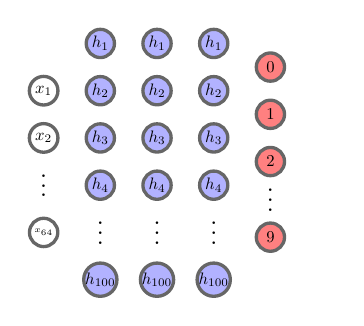
\begin{tikzpicture}[thick,scale=0.6, every node/.style={scale=0.6}][shorten >=1pt,->,draw=black!50, node distance=\layersep]
    \tikzstyle{every pin edge}=[<-,shorten <=1pt]
    \tikzstyle{neuron}=[circle,draw=black!60,fill=black!25,minimum size=17pt,inner sep=0pt, very thick]
    \tikzstyle{missing}=[draw=none, scale=1.5,text height=0.333cm,execute at begin node=\color{black}$\vdots$]
    \tikzstyle{input neuron}=[neuron, fill=white!50,inner sep=2pt];
    \tikzstyle{output neuron}=[neuron, fill=red!50];
    \tikzstyle{hidden neuron}=[neuron, fill=blue!30];
    \tikzstyle{dead}=[draw=none, scale=1.5,text height=0.333cm]
    \tikzstyle{cost neuron}=[neuron, fill=black!30,inner sep=2.4pt];
    \tikzstyle{label neuron}=[neuron, fill=yellow!60,inner sep=1.6pt];
    \tikzstyle{annot} = [text width=4em, text centered]

    % Draw the input layer nodes
    \foreach \name / \y in {1,2}
    	\path[yshift=-1.0cm]
        	node[input neuron] (I-\name) at (0,-\y) {$x_\y$};
    \path[yshift=-1.0cm]
    	node[missing] (I-3) at (0,-3) {};
    \path[yshift=-1.0cm]
		node[input neuron] (I-4) at (0,-4) {\tiny $x_{64}$};
    
    % Draw the hidden layer nodes
    
    \foreach \name / \y in {1,2,3,4}
        \path[yshift=0.0cm]
            node[hidden neuron] (H-\name) at (\layersepSmall,-\y cm) {$h_\y$};
    
    \path[yshift=0.0cm]
            node[missing] (H-5) at (\layersepSmall,-5 cm) {};

    \path[yshift=0.0cm]
            node[hidden neuron] (H-6) at (\layersepSmall,-6 cm) {$h_{100}$};
            
        % Draw the hidden layer nodes
    
    \foreach \name / \y in {1,2,3,4}
        \path[yshift=0.0cm]
            node[hidden neuron] (H-\name) at (2*\layersepSmall,-\y cm) {$h_\y$};
    
    \path[yshift=0.0cm]
            node[missing] (H-5) at (2*\layersepSmall,-5 cm) {};

    \path[yshift=0.0cm]
            node[hidden neuron] (H-6) at (2*\layersepSmall,-6 cm) {$h_{100}$};
            
            
        % Draw the hidden layer nodes
    
    \foreach \name / \y in {1,2,3,4}
        \path[yshift=0.0cm]
            node[hidden neuron] (H-\name) at (3*\layersepSmall,-\y cm) {$h_\y$};
    
    \path[yshift=0.0cm]
            node[missing] (H-5) at (3*\layersepSmall,-5 cm) {};

    \path[yshift=0.0cm]
            node[hidden neuron] (H-6) at (3*\layersepSmall,-6 cm) {$h_{100}$};


	    % Draw the hidden layer nodes
    
  %  \foreach \name / \y in {1,2}
   %     \path[yshift=-0.8cm]
    %        node[hidden neuron] (H-\name) at (4*\layersepSmall,-\y cm) {$h_\y$};
    
%    \path[yshift=-0.8cm]
 %           node[missing] (H-3) at (4*\layersepSmall,-3 cm) {};

 %   \path[yshift=-0.8cm]
  %          node[hidden neuron] (H-4) at (4*\layersepSmall,-4 cm) {$h_{20}$};
            
            
    % Draw the output layer
    
    \foreach \name / \y in {0,1,2}
        \path[yshift=-1.5cm]
            node[output neuron] (O-\name) at (4*\layersepSmall,-\y cm) {$\y$};
    
    \path[yshift=-0.3cm]
            node[missing] (O-4) at (4*\layersepSmall,-4 cm) {};
    
    \path[yshift=-0.1cm]
            node[output neuron] (O-5) at (4*\layersepSmall,-5 cm) {$9$};
    %Draw empty neuron for x- seperation   
    \path[yshift=-0.1cm]
            node[dead] (D-5) at (5*\layersepSmall,-5 cm) {};
            
\end{tikzpicture}
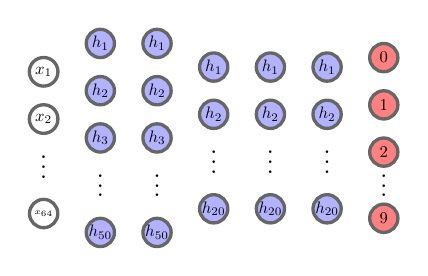
\begin{tikzpicture}[thick,scale=0.6, every node/.style={scale=0.6}][shorten >=1pt,->,draw=black!50, node distance=\layersep]
    \tikzstyle{every pin edge}=[<-,shorten <=1pt]
    \tikzstyle{neuron}=[circle,draw=black!60,fill=black!25,minimum size=17pt,inner sep=0pt, very thick]
    \tikzstyle{missing}=[draw=none, scale=1.5,text height=0.333cm,execute at begin node=\color{black}$\vdots$]
    \tikzstyle{input neuron}=[neuron, fill=white!50,inner sep=2pt];
    \tikzstyle{output neuron}=[neuron, fill=red!50];
    \tikzstyle{hidden neuron}=[neuron, fill=blue!30];
    \tikzstyle{dead}=[draw=none, scale=1.5,text height=0.333cm]
    \tikzstyle{cost neuron}=[neuron, fill=black!30,inner sep=2.4pt];
    \tikzstyle{label neuron}=[neuron, fill=yellow!60,inner sep=1.6pt];
    \tikzstyle{annot} = [text width=4em, text centered]

    % Draw the input layer nodes
    \foreach \name / \y in {1,2}
    	\path[yshift=-0.6cm]
        	node[input neuron] (I-\name) at (0,-\y) {$x_\y$};
    \path[yshift=-0.6cm]
    	node[missing] (I-3) at (0,-3) {};
    \path[yshift=-0.6cm]
		node[input neuron] (I-4) at (0,-4) {\tiny $x_{64}$};
    
    % Draw the hidden layer nodes
    
    \foreach \name / \y in {1,2,3}
        \path[yshift=0.0cm]
            node[hidden neuron] (H-\name) at (\layersepSmall,-\y cm) {$h_\y$};
    
    \path[yshift=0.0cm]
            node[missing] (H-4) at (\layersepSmall,-4 cm) {};

    \path[yshift=0.0cm]
            node[hidden neuron] (H-5) at (\layersepSmall,-5 cm) {$h_{50}$};
            
        % Draw the hidden layer nodes
    
    \foreach \name / \y in {1,2,3}
        \path[yshift=0.0cm]
            node[hidden neuron] (H-\name) at (2*\layersepSmall,-\y cm) {$h_\y$};
    
    \path[yshift=0.0cm]
            node[missing] (H-4) at (2*\layersepSmall,-4 cm) {};

    \path[yshift=0.0cm]
            node[hidden neuron] (H-5) at (2*\layersepSmall,-5 cm) {$h_{50}$};
            
            
	    % Draw the hidden layer nodes
    
    \foreach \name / \y in {1,2}
        \path[yshift=-0.5cm]
            node[hidden neuron] (H-\name) at (3*\layersepSmall,-\y cm) {$h_\y$};
    
    \path[yshift=-0.5cm]
            node[missing] (H-3) at (3*\layersepSmall,-3 cm) {};

    \path[yshift=-0.5cm]
            node[hidden neuron] (H-4) at (3*\layersepSmall,-4 cm) {$h_{20}$};


	    % Draw the hidden layer nodes
    
    \foreach \name / \y in {1,2}
        \path[yshift=-0.5cm]
            node[hidden neuron] (H-\name) at (4*\layersepSmall,-\y cm) {$h_\y$};
    
    \path[yshift=-0.5cm]
            node[missing] (H-3) at (4*\layersepSmall,-3 cm) {};

    \path[yshift=-0.5cm]
            node[hidden neuron] (H-4) at (4*\layersepSmall,-4 cm) {$h_{20}$};
            
     	    % Draw the hidden layer nodes
    
    \foreach \name / \y in {1,2}
        \path[yshift=-0.5cm]
            node[hidden neuron] (H-\name) at (5*\layersepSmall,-\y cm) {$h_\y$};
    
    \path[yshift=-0.5cm]
            node[missing] (H-3) at (5*\layersepSmall,-3 cm) {};

    \path[yshift=-0.5cm]
            node[hidden neuron] (H-4) at (5*\layersepSmall,-4 cm) {$h_{20}$};
            
                
    % Draw the output layer
    
    \foreach \name / \y in {0,1,2}
        \path[yshift=-1.3cm]
            node[output neuron] (O-\name) at (6*\layersepSmall,-\y cm) {$\y$};
    
    \path[yshift=-1cm]
            node[missing] (O-4) at (6*\layersepSmall,-3 cm) {};
    
    \path[yshift=-0.7cm]
            node[output neuron] (O-5) at (6*\layersepSmall,-4 cm) {$9$};
            
\end{tikzpicture}
\caption[NN architectures]{Four different NN- architectures. From left to right, we'll call them \textit{Shallow1}, \textit{Shallow2}, \textit{Deep1} and \textit{Deep2}. White nodes indicate the 64 input neurons. Blue nodes indicate hidden layer- neurons. Red nodes indicate the 10 output neurons.}
\label{NNarchitectures}
\end{figure}
Each of these were trained using the same parameters and their accuracy on test data measured using 4- fold Cross Validation. The results are shown in figure \ref{TinyTableArchitect} below.

\begin{figure}[H]
\centering

\includegraphics[trim=0cm 12.0cm 0cm 0.0cm, clip=true,scale = 0.6]{Architecture_d.pdf}
\caption[NN architectures Accuracy]{Accuracy on test set for Four different NN- architectures: \textit{Shallow1}, \textit{Shallow2}, \textit{Deep1} and \textit{Deep2}.100 batch size, solver ADAM, Activation function LeakyRELU, L2- regularization 0.0001, 4 folds in K- fold Cross validation.}\label{TinyTableArchitect}
\end{figure}


We see that doubling the number of neurons in the single layer perceptron makes some difference, namely increasing the accuracy overall, and in two instances, bringing it all the way up to 99\%. Looking at \textit{Deep1}, we see that adding two more layers of equal thickness to \textit{Shallow1} actually makes the model worse.\\It's first in the thin and deep network architecture \textit{Deep2} that we see considerable change. Despite having more neurons than the 100 neuron single layer perceptron, it makes substantially worse predictions. In this case at least, it's clear that little improvement is made in making the single layer perceptron more complicated.

\subsubsection{Impact of Hidden Layer Activation Function}
Every neuron in the hidden layers of our neural network is equipped with the same activation function. The choice we make ought to influence the numerical stability and convergence of the model. To examine this, we plot the accuracy of the models on test data from 4- fold Cross Validation. Varying over a range of learning rates and number of epochs. The result is shown below in figure \ref{NN_activation}.

\begin{figure}[H]
\centering

\includegraphics[trim=0cm 12.0cm 0cm 0.0cm, clip=true,scale = 0.6]{Activation_function_d.pdf}
\caption[NN Hidden layer Activation]{Four different hidden layer activation functions. Number of epochs on the y- axis, learning rate $\eta$ on the x- axis. Accuracy in proportion of correctly classified digits in test set of each model over 4 folds. Batch size 100, L2 regularization parameter 0.0001, solver = ADAM and architecture [100, 100, 50, 50].}\label{NN_activation}
\end{figure}

A score close to 0.1 is indicative of a random guess with the most likely candidate for failure being numerical instability or extremely slow convergence. Slow convergence seems to be the case for the sigmoid function which has very poor results for the smallest learning rate. For the next smallest learning rate we see an improvement with a ten fold increase in the number of epochs followed by little improvement with a doubling and quadrupling.\\ RELU and LeakyRELU seems to suffer from numerical instability at the largest learning rate with a much more aggressive difference from the next largest learning rate compared to the tanh activation function.\\ LeakyRELU for this particular configuration of solver, architecture and regularization parameter, gives the best score of 98\% for learning rates on the order of $10^{-3}$ and 200 epochs.

\subsection{Multinomial Logistic Regression for Digit Classification}

\subsubsection{What is wrongly classified?}
Our model does make wrong predictions. It's worthwhile to examine what images it classifies wrongly in order to understand where the problem arises. Figure \ref{Digits} below shows a random sample of four digits that were wrongly classified with their attached labels and the prediction of the model.

\begin{figure}[H]
\centering

\includegraphics[trim=6cm 5.0cm 12cm 5.0cm, clip=true,scale = 0.5]{Wrong_predictions_LogReg.pdf}
\caption[Wrongly classified Digits]{Random selection of 4 wrongly classified handwritten digits in the testing set. Classification was made using multinomial logistic regression with stochastic gradient descent. Using 10 epochs and a learning rate of $0.001$. Model accuracy was 95.56\%.}\label{Digits}
\end{figure}

Arguably, one of the benchmarks by which we should measure the success of our algorithm, is human judgement. Recruiting the aid of an impartial judge, who had not seen either the labels or predictions. They determined from left to right in figure \ref{Digits}, that the digits looked like 9, 1, 5 and 1 respectively. The first and last of which are wrong according to their labels. With this in mind we can conclude that a not insignificant portion of the wrongly classified images lack the pixel resolution needed to meaningfully distinguish them from another digit.

\subsubsection{Impact of Learning Rates}
We want to examine the role that the learning rate plays in the testing accuracy of our models. Using 150 epochs and a batch size of 1, we get figure \ref{Acc_to_LR} below.

\begin{figure}[H]
\centering

\begin{tikzpicture}
    \node[anchor=south west,inner sep=0] at (0,0) {\includegraphics[trim=0cm 0.2cm 0.5cm 0.8cm, clip=true,scale = 0.65]{e_test_accuracy_over_learning_rate.pdf}};
    \draw[red,dashed] (1.9,7.14) -- (13.7,7.14);
    \draw[blue,dashed] (4.55,0.9) -- (4.55,7.14);
\end{tikzpicture}

%\includegraphics[trim=1cm 0.4cm 1cm 0.8cm, clip=true,scale = 0.6]{e_test_accuracy_over_learning_rate.pdf}
\caption[Classification accuracy to learning rate (Softmax Regression)]{Multinomial logistic regression with stochastic gradient descent. Classification accuracy on the test set as a function of learning rate. Using 150 epochs and a bach size of 1.}\label{Acc_to_LR}
\end{figure}
We see that there's a stable region between $\eta = 10^{-4}$ and $\eta = 1$ that results in relatively high accuracies. We expect that too large learning rates should prevent the algorithm from converging on an optimum, instead oscillating around it. Too small learning rates may not converge by the time 150 epochs have elapsed. With this in mind, we should expect to see the graph peak at lower learning rates if the algorithm is given more epochs for convergence. We can see this effect in figure \ref{Acc_to_LR_2} below.

\begin{figure}[H]
\centering
\begin{tikzpicture}
    \node[anchor=south west,inner sep=0] at (0,0) {\includegraphics[trim=0cm 0.2cm 0.5cm 0.8cm, clip=true,scale = 0.65]{e_test_accuracy_over_learning_rate2.pdf}};
    \draw[red,dashed] (1.4,6.03) -- (9.5,6.03);
    \draw[blue,dashed] (2.78,0.8) -- (2.78,6.03);
\end{tikzpicture}
%\includegraphics[trim=0cm 0.2cm 0.5cm 0.8cm, clip=true,scale = 0.65]{e_test_accuracy_over_learning_rate2.pdf}
\caption[Classification accuracy to learning rate (Softmax Regression)]{Multinomial logistic regression with stochastic gradient descent. Classification accuracy on the test set as a function of learning rate. Using 400 epochs and a bach size of 1.}\label{Acc_to_LR_2}
\end{figure}
Here, the threshold for an accuracy above 90\% has shifted towards the smaller learning rate with an increase in the number of epochs.


\subsubsection{Comparing Implementation to Scikit- learn}
Using a learning rate $\eta = 0.0001$ and $500$ epochs on $6$ independent runs. Comparing the Scikit- learn implementation with our own implementation of Logistic regression with Stochastic regression we get the results in table \ref{Softmax_sci_v_us}.
\begin{table}[H]
\caption[Classification accuracy comparison to Scikit- Learn]{Own implementation of Softmax regression with stochastic gradient descent compared to a Scikit- Learn implementation using the LBFGS. Classification accuracy on a test set randomized between each run. Using 500 epochs for both methods and a learning rate of 0.0001 and batch size of 1 for the SGD solver.}
\centering
\begin{tabular}{|l|l|l|}
\hline
Run & Softmax Regression with SGD & Scikit Logistic Regressor with LBFGS \\ \hline
1   & 97.22\%                     & 95.83\%                              \\ \hline
2   & 95.83\%                     & 94.17\%                              \\ \hline
3   & 97.22\%                     & 96.94\%                              \\ \hline
4   & 96.67\%                     & 95.56\%                              \\ \hline
5   & 94.44\%                     & 95.56\%                              \\ \hline
6   & 96.11\%                     & 96.67\%                              \\ \hline
\end{tabular}\label{Softmax_sci_v_us}
\end{table}
The key difference between these two different implementations is the use of LBFGS solver utilized by the LogisticRegression function (default setting) in Scikit- learn. We can see that their accuracy is roughly the same across runs. This seems to indicate that we have correctly implemented a Softmax regressor using SGD.

\section{Conclusion}
We have seen that stochastic gradient methods are well suited to approximate the ideal OLS and Ridge parameters, with ADAM being able to achieve a test MSE only 20\% higher at 1000 epochs with a batch size of 16 compared to the ideal Ridge parameter. However, the analytical solution is always to be preferred, given it exists. \\ 
As can be see in the preceding section on regression, getting results that surpass Ridge Regression and OLS is not difficult with a FFNN, which shows that neural networks are well suited for regression problems. However, finding the ideal parameters is no easy task, as there are a lot of activation functions, gradient methods and parameters to choose. There is also the aspect of time - higher epochs lead to superior results, but the error reduces extremely slowly as the number of epochs grows exponentially \citep{handsOnMachineLearning}. For the regression problem, we found, with help of the sigmoid function, that ADAM worked best as stochastic gradient method, whereas the tanh activation function worked best as activation function (with 2 hidden layers), giving $60\%$ of the test MSE that OLS produces. However, we observed that the Rectifier activation functions, especially LeakyReLU, perform better for deeper neural networks, and we hence suppose that the error can be further reduced by using LeakyReLU as activation function with more epochs. Ultimately however, the Neural Network cannot hide the fact that regression on terrain data cannot yield exact results because of the complicated shape \& the fact that sampling with so few points cannot be correct. \\\\

In the classification problem we find that the thick and shallow network architectures i.e. \emph{Shallow1} and \emph{Shallow2}, produce the best results over a range of epochs and learning rates, keeping everything else constant. This suggests that the particular problem of classifying an $8\times 8$ grid of pixels, does not benefit from the addition of more hidden layers with the number of epochs we're considering.\\We found that, within the range of epochs we looked at and the particular choice of architecture, LeakyRELU produced models with the highest accuracy of 99\%, with both tanh and RELU following closely behind with consistent accuracies of 97\%. Sigmoid, at least for this number of epochs produced considerably worse results.\\In Multinomial logistic regression, we looked at some of the wrongly classified digits and found at least some of them to be indistinguishable from another digit, suggesting that the limited pixel value of the dataset is reducing the feasible accuracy of our models. Looking at how we might interpret accuracy scores when tweaking learning rate and the number of epochs in our parameter space, we found (unsurprisingly) that allowing for more epochs makes lower learning rates perform better.\\As for whether logistic regression or neural networks are better for digit classification, we saw clearly better results when using neural networks, although the time required for convergence was consistently much higher for neural networks.\\

One way to improve on this is report is to implement proper cutoff procedures for numerical instability to reduce run time, since bad parameters give overflow errors and hence unusable results. This includes stopping after the test accuracy stops improving or when the train accuracy is 1. It is absolutely possible to improve this implementation's run time by being more strict in using vectorized code and avoiding unnecessary memory allocations by doing in-place manipulation of data (or writing the code in a compiled language such as C). Different type of Neural Networks give much improved results for classification. With a deep FFNN and deformed training images, it is possible to get the test error to 0.35\% and below \citep{betterThanUs}. Using Convolutional Neural Networks, it is possible to get the error down to 0.21\% \citep{Convolution}, and it looks like there is still room for improvement.  We are quite convinced that we did not find optimal parameters, as we did not explore the full parameter space of these methods. Our search search was mainly restricted to a simple grid search and a limited number of epochs and hidden layers. We also did not implement the full MNIST dataset, but only a reduced version thereof, and it would be interesting to see how well our simple network performs on the full data, both in terms of speed and quality. 
\section{Appendix}
\subsection{Proof that Softmax reduces to the Logistic function for m=2}\label{ProofSoftmaxToLogistic}

Consider the Softmax function for $m=2$ categories

\begin{equation}
\textbf{a} = \frac{1}{ \exp(\textbf{W}_{[1,:]}\cdot \textbf{x}^T)  + \exp( \textbf{W}_{[2,:]} \cdot \textbf{x}^T ) }
\begin{pmatrix}
\exp( \textbf{W}_{[1,:]} \cdot \textbf{x}^T) \\
\exp( \textbf{W}_{[2,:]} \cdot \textbf{x}^T)
\end{pmatrix}
\end{equation}
We can multiply both sides of the fraction by $\exp(- \textbf{W}_{[2,:]} \cdot \textbf{x}^T)$ to get
\begin{equation}
\textbf{a} = \frac{1}{ 1  + \exp( (\textbf{W}_{[1,:]} -\textbf{W}_{[2,:]})\cdot \textbf{x}^T) }
\begin{pmatrix}
\exp( (\textbf{W}_{[1,:]} -\textbf{W}_{[2,:]})\cdot \textbf{x}^T) \\
\exp( \vec{0})
\end{pmatrix}
\end{equation}
We can now simply rename this weight parameter as $\textbf{W}_{[1,:]} -\textbf{W}_{[2,:]} = -\textbf{W}$ giving us
\begin{equation}
a = \begin{pmatrix}
\frac{\exp( -\textbf{W}\cdot \textbf{x}^T)}{1+\exp( -\textbf{W}\cdot \textbf{x}^T)} \\
\frac{1}{1+ \exp( -\textbf{W}\cdot \textbf{x}^T)}
\end{pmatrix} = \begin{pmatrix}
1-\frac{1}{1+\exp( -\textbf{W}\cdot \textbf{x}^T)} \\
\frac{1}{1+ \exp( -\textbf{W}\cdot \textbf{x}^T)}
\end{pmatrix} 
\end{equation}
which is the same as the activation function for logistic regression.
\subsection{Figures}
\begin{figure}[H]
\centering
\includegraphics[width=0.95\textwidth]{Ridge_error_SGD.pdf}
\caption[Relative Test MSE with different SGD methods for Ridge]{Relative Test MSE  ($\frac{MSE_{SGD}}{MSE_{analytical}})$ for the simple SGD method, RMSProp and ADAM and as functions of the learning rate $\eta$ and the regularization parameter $\lambda$. $N=2000$, the polynomial degree used is $deg=20$, where OLS fails. The batch size is 16, the number of epochs is 1000. Values exceeding 10 were removed, explaning the grey parts. No bootstrapping or cross-validation was performed.} \label{fig:DifferentSGDRIDE}
\end{figure}

\begin{figure}[H]
\centering
\includegraphics[width=1.05\textwidth]{scikit_own_2b1_logisticsgd200010.pdf}
\caption[Scikit-learn  and own FFNN with 2 layers, degree 20]{Train and test MSE \underline{divided by 1000} as function of the learning rate $\eta$ and the regularization parameter $\lambda$ for our own Neural Network and Scikit-learn 's MLPRegressor function. We used 2000 data points (randomly selected), a polynomial degree of 20, a batch size of 200, 1000 epochs, two hidden layers with 100 neurons each, simple SGD as gradient descent method and the sigmoid function as activation function between the layers. Values exceeding 100,000 are excluded from the plot. We used 5-fold Cross Validation to estimate the errors.} \label{fig:ScikitLearn_3}
\end{figure}
\begin{figure}[H]
\centering
\includegraphics[width=1.0\textwidth]{4_layers.pdf}
\caption[4 hidden layers, 100 epochs]{Test MSE \underline{divided by 1000} as function of the learning rate $\eta$ and the regularization parameter $\lambda$ for our own Neural Network using ADAM. We used 2000 data points (randomly selected), a polynomial degree of 10, a batch size of 200, 1000 epochs, 4 hidden layers with respectively 100, 100, 50 and 50 neurons and the activation function stated in the title between the layers. Values exceeding 100,000 are excluded from the plot. We used 5-fold Cross Validation to estimate the errors.} \label{fig:4layers}
\end{figure}
\begin{figure}[H]
\centering
\includegraphics[width=1.0\textwidth]{2_layers_short.pdf}
\caption[4 hidden layers, 100 epochs]{Test MSE \underline{divided by 1000} as function of the learning rate $\eta$ and the regularization parameter $\lambda$ for our own Neural Network using ADAM. We used 2000 data points (randomly selected), a polynomial degree of 10, a batch size of 200, 100 epochs, two hidden layers with 100 neurons each and the activation function stated in the title between the layers. Values exceeding 100,000 are excluded from the plot. We used 5-fold Cross Validation to estimate the errors.} \label{fig:2layers}
\end{figure}


\bibliographystyle{plain}
\bibliography{references}
\end{document}
